\hoofdstuk{Background}
\paragraaf{Lunatech Research B.V}
Lunatech provides application development services, completely based on open-source web and Java technologies and open standards. They are early adopters of new technology, and use cutting-edge frameworks and tools to give themselves the advantage in software development. To stay up-to-date, their developers have the opportunity to research, try new technologies and contribute to open-source projects. The company is dominated by software developers. Everyone (except the director) writes code, on top of which some staff have a secondary management role, and the staff who will deliver a project interact with the customer directly.

\paragraaf{Rotterdam University of Applied Sciences (Hogeschool Rotterdam)}
Rotterdam University is one of the major Universities of Applied Sciences in the Netherlands. Currently almost 30,000 students are working on their professional future at our university.
The university is divided into eleven schools, offering more than 80 graduate and undergrad- uate programmes in seven fields: art, technology, media and information technology, health, behaviour and society, engineering, education, and of course, business.\cite{HogeschoolRotterdam2012}

\paragraaf{Stager}
In 2011, live music venue WORM - Instituut voor Avantgardistische Recreatie hired Lunatech to build Stager, a modern web-based resource planning and ticketing application to help manage live music events. Lunatech took the opportunity to use the relatively new Play framework to build a web application with an HTML5 and Java architecture. Stager has broad requirements ranging from high performance and security for the public ticket sales component, high usability for the internal resource planning component that will be used for hours a day by employees and being open to enhancements in the future for new customers.

\subparagraaf{WORM}
WORM is een instituut voor avantgardistische recreatie te Rotterdam, bestaande uit een kunstenaarscollectief, een podium met winkel en een Parallelle Universiteit (DIY-werkplaatsen 
voor film, muziek en media). Geboren onder de sterren van punk, dada, fluxus, situationisme en futurisme is WORM uitgegroeid tot een eigengereide organisatie die de ‘Do-It-Yourself’ mentaliteit van hun voorouders combineert met ultra-pragmatisme, liefde voor techniek(en) en goede boekhouding. De output van WORM is film, radio, concerten, cursussen, party's, publicaties, performances, web-projecten, installaties, workshops en een op­eenhoping van tactiele media en internet. WORM focust zich (blijmoedig en toch serieus) op avantgarde, middelenschaarste en opensource.


\hoofdstuk{Mobile platforms}

\paragraaf{Introduction}
% per platform: van wie is het, wat is de geschiedenis, waar wordt het gebruikt, welke achterliggende techniek drijft het?
The following chapter presents a concise overview of current mobile operating systems for mobile platforms, specifically smartphones and tablets.

A smartphone can be defined as a smart phone is a next-generation, multifunctional cell phone that provides voice communication and text-messaging capabilities and facilitates data processing as well as enhanced wireless connectivity.\cite{Ni2006}

\subparagraaf{Apple iOS}
iOS is a proprietary mobile operating system, developed by Apple Inc. It was originally released in 2007 for the iPhone and iPod Touch. iOS also became the main operating system of the iPad and Apple TV.

\subparagraaf{Google Android}
Android is a opensource mobile operating system, developed by the Open Handset Alliance, led by Google and other companies.\cite{Inc.2012}

\subparagraaf{BlackBerry OS}
BlackBerry OS is a proprietary mobile operating system, developed by RIM\emph{(Research In Motion)} for its line of BlackBerry mobile devices.

\subparagraaf{Windows Phone 7}
Windows Phone 7 is a mobile operating system, developed Microsoft as a succesor to its Windows Mobile platform.

\subparagraaf{Java ME}

\subparagraaf{Symbian}

\paragraaf{Marketshare and trend}


\begin{centering}
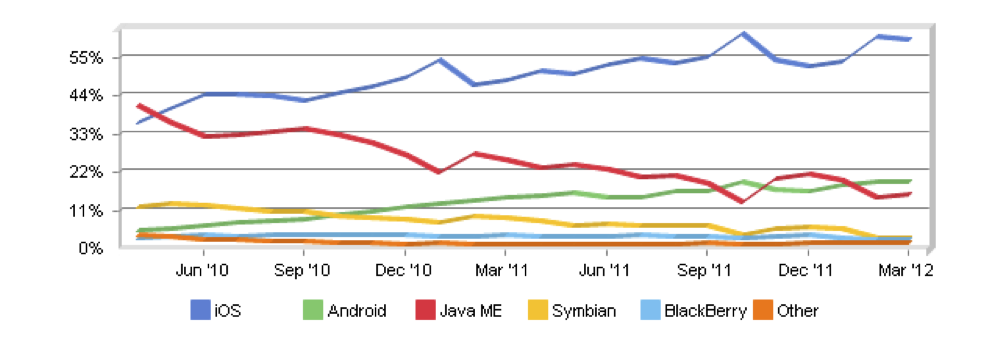
\includegraphics[scale=0.5]{images/marketsharetrendsApril10Tomay12.png}\\{World wide mobile OS Marketshare trends, April 2010 up to may 2012}\\
\end{centering}


\begin{centering}
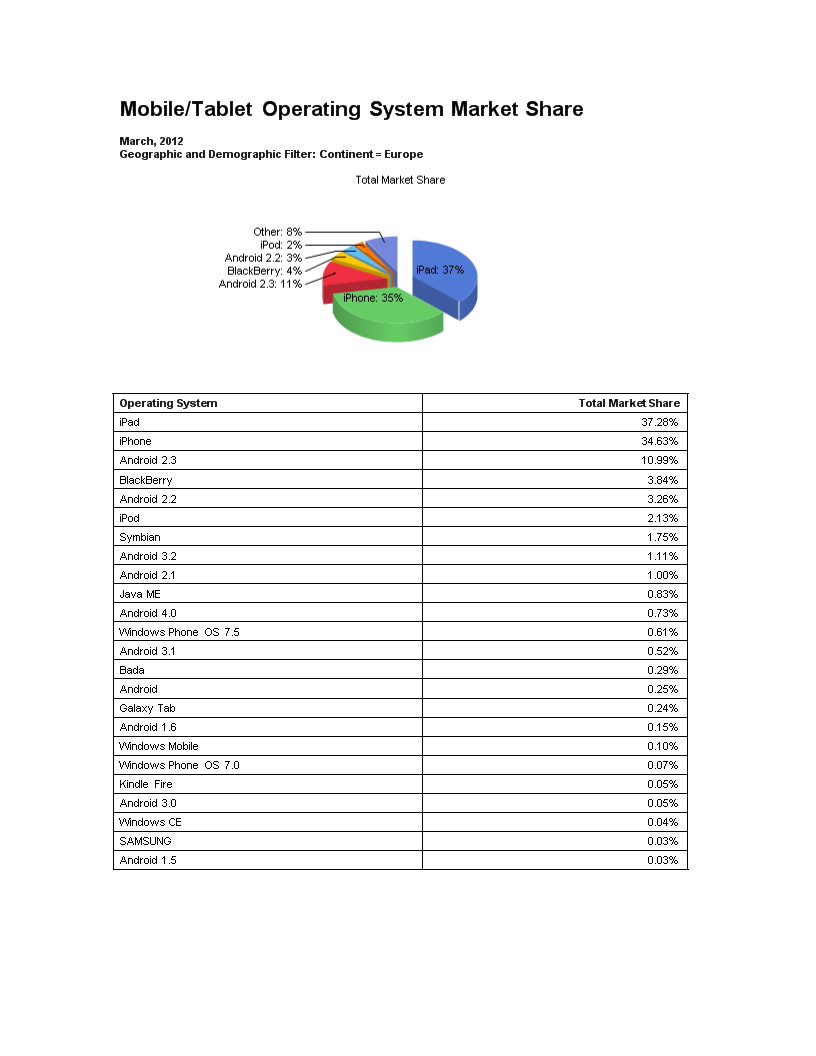
\includegraphics[scale=0.5]{images/netmarketshare_march2012.png}\\
\end{centering}

\begin{tabel}{|>\R p{\Procent{25}} | >\R p{\Procent{25}} |}{vbx}{Marketshare in the european continent as of march 2012\cite{Netmarketshare2012}}
\hline
\bf{Operating System} & \bf{Total \% Market Share}\\
\hline \hline
iOS & 74.04\\
Android & 18.36\\
BlackBerry & 3.84\\
Symbian & 1.75\\
Java ME & 0.83\\
Windows Phone & 0.68\\
Bada & 0.29\\
Windows Mobile & 0.14\\
Kindle & 0.05\\
Samsung & 0.03\\
LG & 0.01\\
ZTE & 0.00\\
Palm & 0.00\\
\hline
\end{tabel}



\hoofdstuk{Defining native}
\paragraaf{Intoduction}
The following chapter will define the \emph{native look-and-feel}.

\paragraaf{Native mobile applications}
A native application is by definition an application inherent to the platform it was build for using techniques proprietary to the platform. For example, an iOS application is native when written in Objective-C and an Android app is written in Java.  Native apps are typically fast can can acces the devices n

\subparagraaf{The native look-and-feel}
When written in the native framework for a platform an mobile application receives acces to the available public libraries of the platform. These libraries include the UIKit\emph{(on iOS)} which provides the developer with a pre fabricated set of user interface components. These can be seen as the buildingblocks for the graphical userinterface on that platform. When used, the general style of the mobile application gains homogeneity to the overal user interface design of the platforms operating system. This gives an application its native look, which in turn participates to the native feel.

%with a feeling of recognition when using the application, userinterface elements work as they expected based upon experience with using the operating system.

The native feel of a mobile application can be defined as the in the speed which the userinterface elements, the responsiveness of userinterface elements to touch events, and finally smoothness of the animation in which the userinterface elements are moved.
A native mobile application has the advantage to hardware acceleration. This means its code has been precompiled and directly executed by the device CPU. As a result of this the userinterface feels smooth.
 	

\paragraaf{Alternative mobile application types}
\subparagraaf{Web applications}
A mobile web application is an application developed with web technologies as Javascript and HTML5 with CSS3. It is in fact nothing more than a website designed to fit on mobile devices, often they resemble the style of a native app rather than a traditional website. Often these application are build with a Javascript library to add support for scrolling and handling touch events. These touch events are handled via widgets, userinterface elements which provide the user with components composed similair to the native components. Examples of these libraries include jQtouch, SenchaTouch.


\subparagraaf{Hybrid applications}
A hybrid application in mobile development refers to an application which use a native \emph{shell} to wrap a web app. There are generally two forms of native shells,  the first is  webview and second a native framework which exposes a javascript API to provide the web app access to otherwise native API's.

\subparagraaf{Webviewbased hybrid applications}
A webviewbased hybrid app is nothing more as a webbased mobile application wrapped in a webview. A webview is a view or element which is acts like a browser would, e.g. it is able to render HTML and run javascript.  It is readily available in the native libraries. The advantage of a webviewbased hybrid app over an normal web app is that it can be published via the devices native app publishing platforms. e.g. a webviewbased hybrid app targetted for the iPhone can be placed in the Apple appstore. 

Worklight is an example of a framework which can be used to develop webviewbased hybrid applications.

\subparagraaf{Mixed hybrid applications}
A Mixed based hybrid app is a webviewbased app build upon a framework which provides a Javascript API to allow the app access to otherwise native API's. The framework is written in the platforms native programming language, this provides the possibility to access the native API, such as reading contact list, composing of SMSes, full access to the location API, etc.

PhoneGap is an example of a framework which can be used to develop mixed hybrid applications.

\paragraaf{Comparison}
Web apps - Quick and cheap to develop. Written entirely in HTML5, CSS and JavaScript. Executed by the mobile
browser and therefore cross - platform by default, but less powerful than native apps.
 
Hybrid Apps (Web) - The app's source code consists of web code executed within a native wrapper that is provided by a framework.
 
Hybrid Apps (Mix) - The developer augments the web code with native language to create unique features and
access native APIs that are not yet available via JavaScript, such as AR, NFC and others.
 
Native Apps - Platform-specific. Requires unique expertise and knowledge. Pricey and time consuming to develop but
 delivers the highest user experience of all approaches.

\begin{centering}
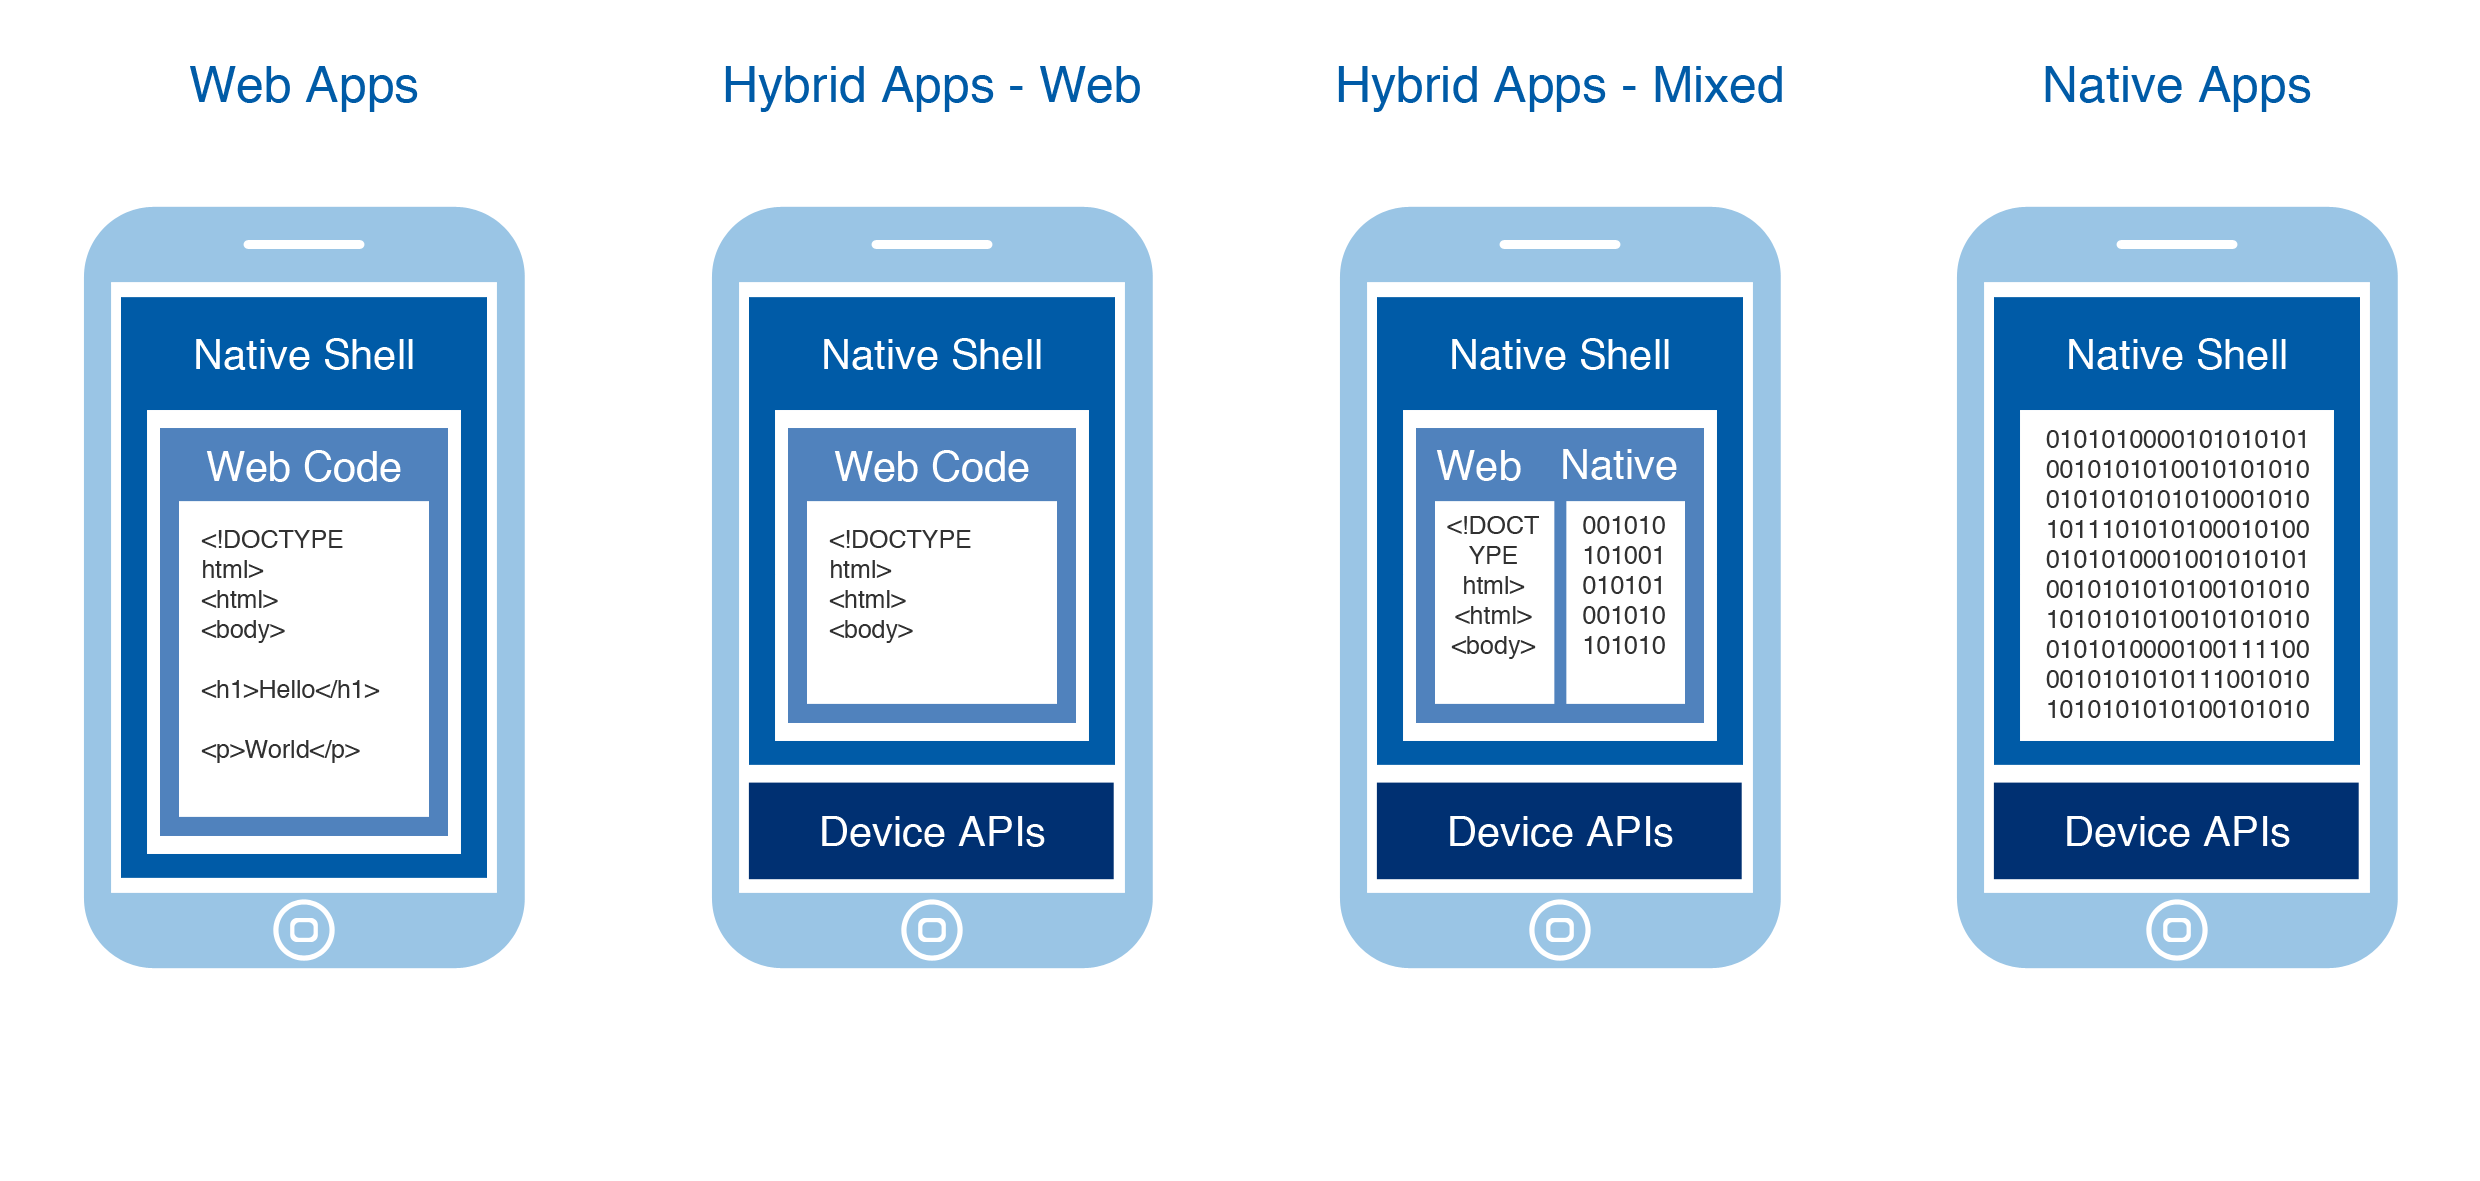
\includegraphics[scale=0.5]{images/apptypesdefined.png}\\{label x}\\
\end{centering}

\hoofdstuk{Exsisting solutions to Cross-platform Mobile Application Development}
\paragraaf{Introduction}
\paragraaf{PhoneGap}
\paragraaf{Appcelerator Titanium}
\paragraaf{Rhodes}
\paragraaf{Worklight}
\paragraaf{MoSync}
\paragraaf{Sencha Touch}
\paragraaf{jQTouch}
\paragraaf{Comparison}

\hoofdstuk{Developing cross-platform native applications with Titanium}
\paragraaf{Inner workings}

\hoofdstuk{Case study}
\paragraaf{Stager app}
\paragraaf{Stager app requirements}
\subparagraaf{Events}
\subparagraaf{Notifications}
\subparagraaf{Tickets}
\subparagraaf{Mobile payment}


%\paragraaf{Titanium modules}
%\paragraaf{Stager service modules}









